\chapter{Proof of concept}

This chapter describes the design, manufacturing and testing of the proof of concept hardware.
Focus is put on verifying, where possible, the simulation results from chapter \ref{chap:concept}.
During the test phase there might be multiple iterations to solve problems found during the tests.
These modification will be described and tested.
At the end of this chapter there should be enough confidence in the working of the system to start with a prototype design.

\section{Antenna}
\label{sec:antenna_proof}

The antenna is elevated above the ultrasonic transducer. It is important to centre the antenna lens and the transducer to make sure their axis align. For this purpose the transducer is centred on a circular mounting plate. The antenna is placed above the transducer by connecting it to two risers which are placed at fixed points in the mounting plate. The result is the antenna concept shown in Figure~\ref{fig:proto_ant}. The two risers could give the antenna a blind spot, later on we test if the risers have influence on the transmitting and receiving characteristics.
  Note that in this design the mechanical connection to the Zebro is not yet implemented. The final design with mechanical interface will be presented in the chapter describing the prototype, section \ref{sec:antennamech}.

\begin{figure}[H]
\centering
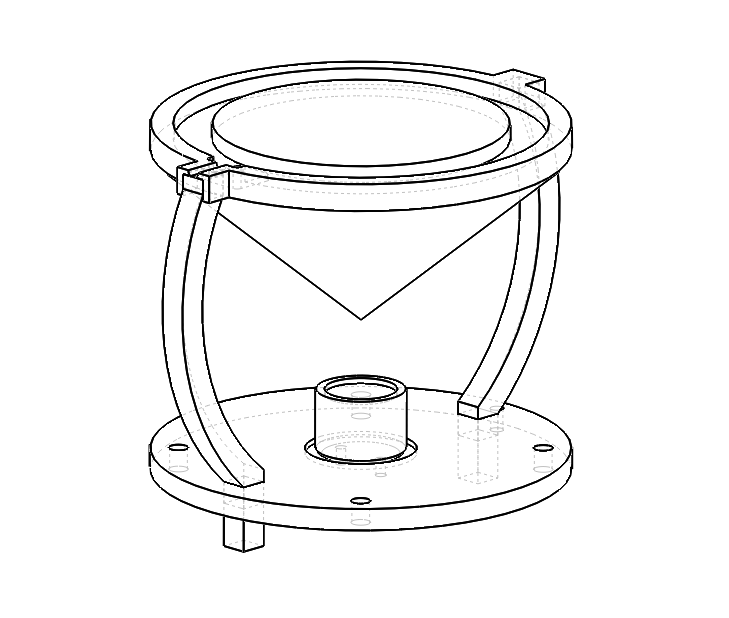
\includegraphics[width=0.6\textwidth]{Figures/proto_ant.PNG}
\caption{Proof of concept version of the ultrasonic antenna}\label{fig:proto_ant}
\end{figure}

Using that the beam pattern of the transducer is \SI{50}{\degree} we can find the distance between transducer and antenna for which the entire beam is incident on the antenna lens. Using the Zebro team 3D printer we made 2 copies of the antenna design, see Figure~\ref{fig:3D_ant}, to use for the proof of concept tests.

\begin{figure}[H]
\centering
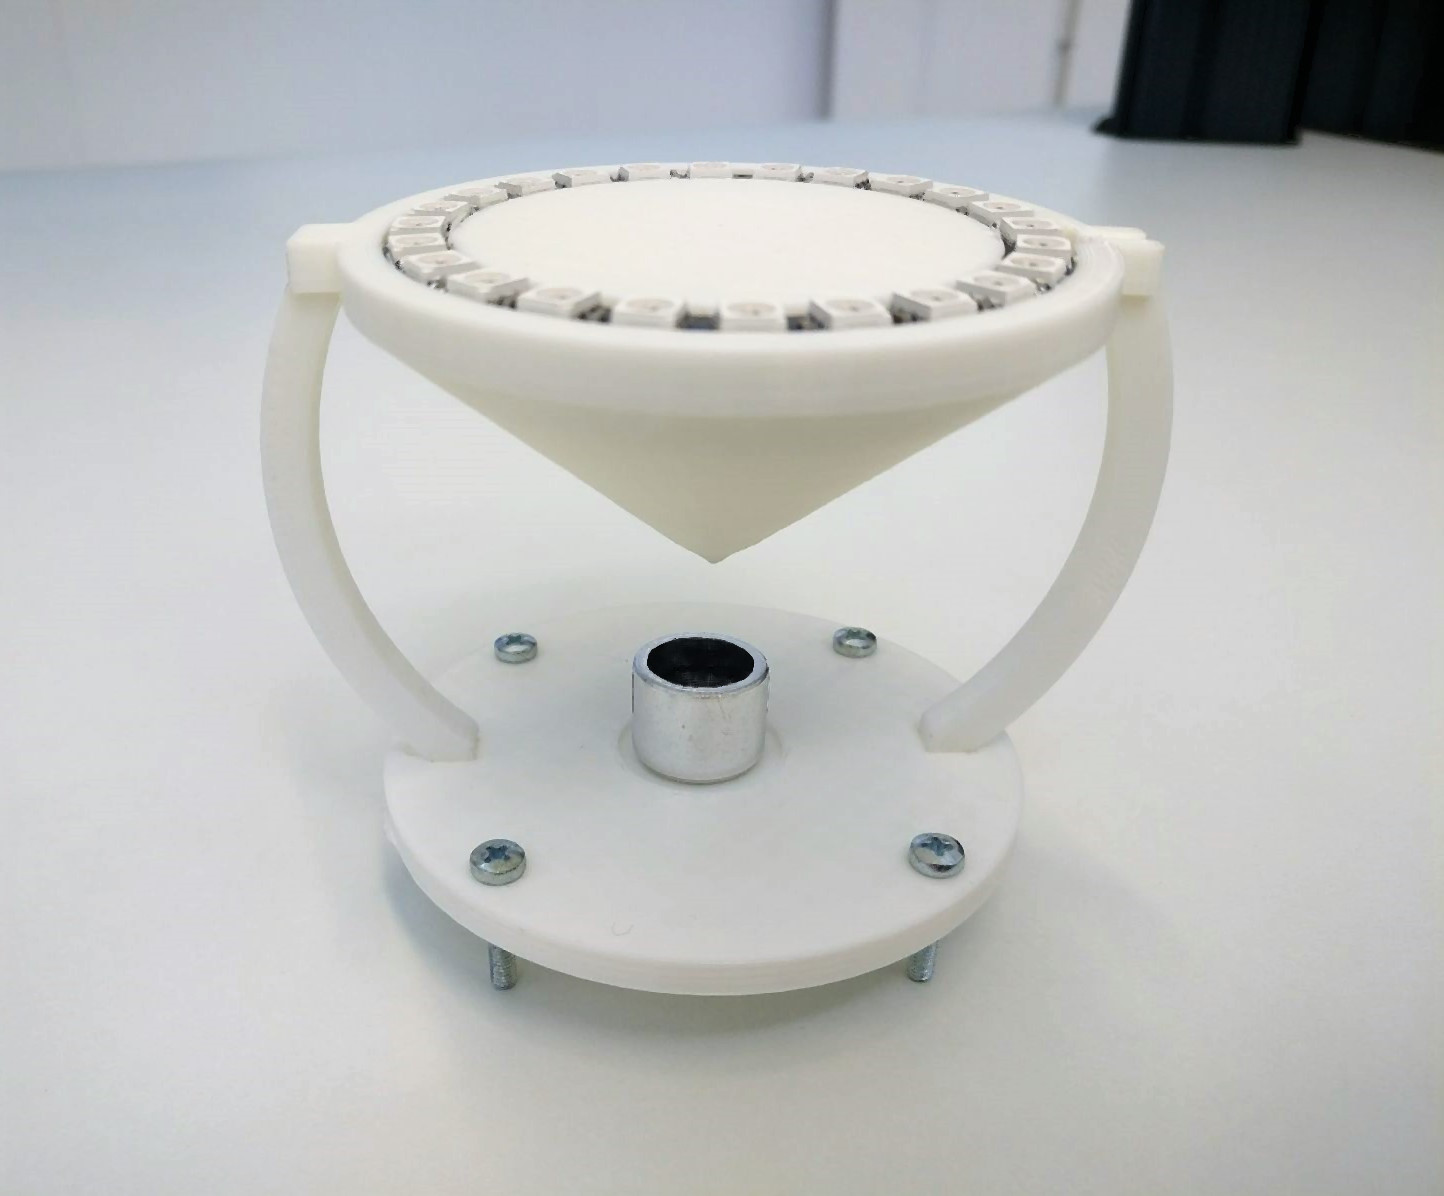
\includegraphics[width=0.6\textwidth]{Figures/3D_ant.jpeg}
\caption{3D printed proof of concept version of the antenna}\label{fig:3D_ant}
\end{figure}

The transmitter and receiver circuits can be connected to the bottom side of the mounting plate. The LED ring on top of the antenna is for human robot interaction purposes and can be used for system debugging and testing.


\section{Protoboard}

The circuit of Figure~\ref{fig:receivecircuit} is made on a protoboard as can be seen in Figure \ref{fig:protoboard}. The components used on the protoboard are the components that were available in the Tellegenhall. For the operation amplifiers we used the LM741 \cite{LM741}
, for the comparators we used a LM339 and  a LM311. The rest of the components are normal resistors and capacitors. For the signals and power sources are cables soldered to the circuit. From left to right on the lower line in the circuit board, are the first and second stage amplifiers visible. Next to the amplifiers is the first stage comparator visible and on top the second stage comparator. On the board is also a potentiometer visible, because of this we can tune the amplification of the operational amplifier.


\begin{figure}[H]
\centering
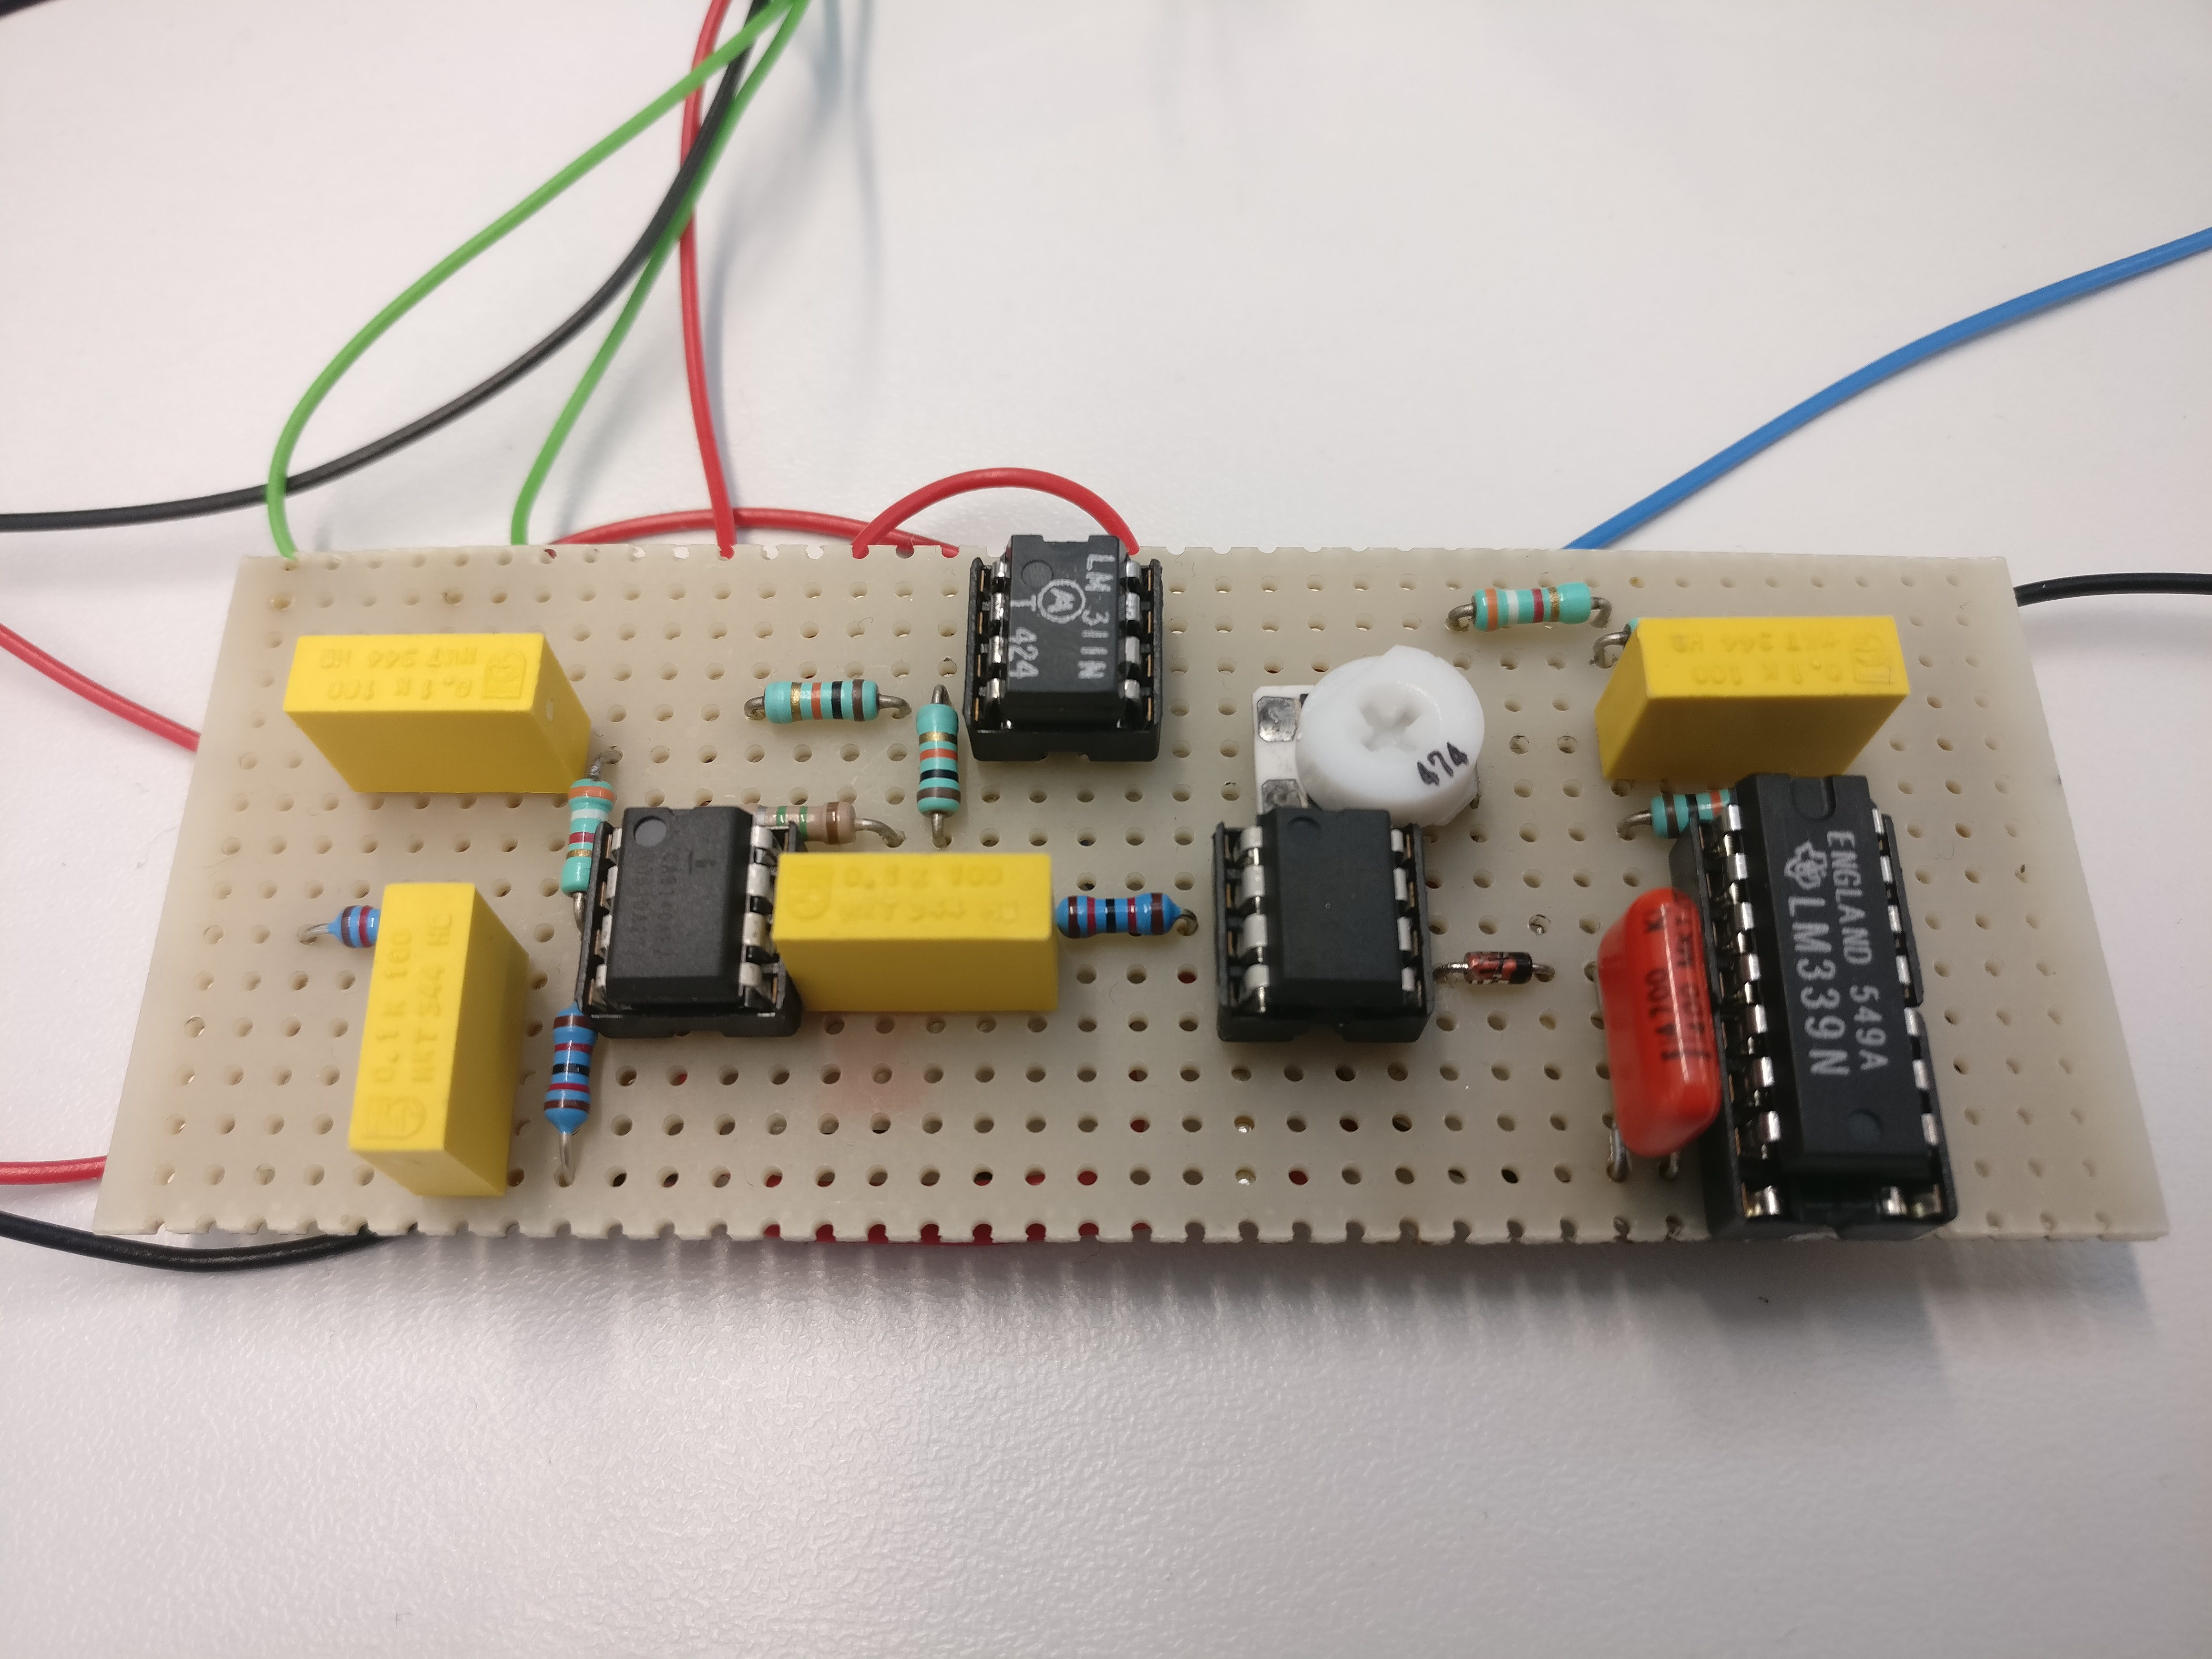
\includegraphics[width=0.6\textwidth]{proof_proto.jpg}
\caption{Proto board for the proof of concept receiver and detector circuit}\label{fig:proto}
\label{fig:protoboard}
\end{figure}

The protoboard of the transmitter circuit is simple, because it is a single MIC4428 \cite{MIC4428}
 IC, only the ultrasonic transceiver is connected to it and the power and signal wires.

\section{Test plan}
The first test is to measure the internal signals of the circuit.
Using an oscilloscope we measure the signal at several points: the input, after each amplification stage, in the peak detection circuit and at the output to verify the correct working of the circuit.
In this test stage we check for production errors such as short circuits and check the component selection.

For the proof of concept tests the communication subsystem is not yet implemented.
This means that we cannot test the full concept as described in chapter~\ref{chap:concept} since we lack the required RF message.
We can however test the generation and accuracy of the $US_{detect}$ signal as seen in Figure~\ref{fig:ultra3}.
The $US_{detect}$ signal must have a clear distinction between a high (no pulse received) and low state (pulse received).
This change from high to low happens when the transducer receives a ultrasonic signal.

To test the circuit we connect it to a transducer placed in the reflecting antenna (Figure~\ref{fig:3D_ant}).
The output of the receiver circuit is the $US_{detect}$ signal.
To simulate the transceiver we power the MIC4428 \cite{MIC4428}
H-bridge driver IC with a power supply and use the signal generator to simulate the \SI{40}{\kilo\hertz} PWM wave output of the micro controller (see Figure~\ref{fig:ultra3}).
The output of the bridge driver IC is connected to a second ultrasonic transducer.

To see the effect the surroundings have on the distance measurements and thus on the $US_{detect}$ signal we perform the test in different set-ups:

\begin{itemize}
\item
Direct orientation with no reflecting surfaces or obstacles near the transmitter and receiver.
\item
The transmitter is placed close to a reflecting surfaces creating multiple paths from the transmitter to the receiver.
The reflecting surfaces are placed such that the extra paths are close in length to the original path.
\item
The transmitter and receiver are placed 7 meters apart with multiple obstacles, such as chairs and members of our bap group, in the direct path.
\end{itemize}

Using an oscilloscope we measure the $US_{detect}$ signal at the output of the receiver circuit.
By setting to oscilloscope to trigger at a falling edge we can visualise the change in the $US_{detect}$ signal.
The resulting measurements are given, and discussed, in the next section.

\section{Results}

When the receiver circuit receives a signal we see the expected \SI{4.5}{\volt} with the incoming signal modulated over it at the receiver input.
The incoming signal is, depending on the distance between transmitter and receiver, in the order of a few millivolt.
The signal is amplified by the first and second stage resulting in a $9V_{p-p}$ sinusoidal wave with an offset of \SI{4.5}{\volt} at the output of the second stage.

When the receiver circuit is not receiving we noticed something strange, instead of the \SI{4.5}{\volt} DC we would expect we see an sinusoidal wave at the output of the second stage.
The origin of this signal is the first amplifier.
While the first amplifier stage has \SI{4.5}{\volt} DC on both input pins it's output is a sinusoidal wave.
We assume that this signal is a noise signal resulting from a bad choice of operational amplifiers.
Since the circuit now generates a sinusoidal wave in both the receiving (intended) and not receiving (noise) state it's impossible to detect an ultrasonic pulse. When receiving an ultrasonic pulse we noticed that the amplification was not the amplification we expected, the amplification was lower.
Modifications need to be made to remove or filter this noise signal and get a higher op-amp amplification.


\begin{figure}[H]
\centering
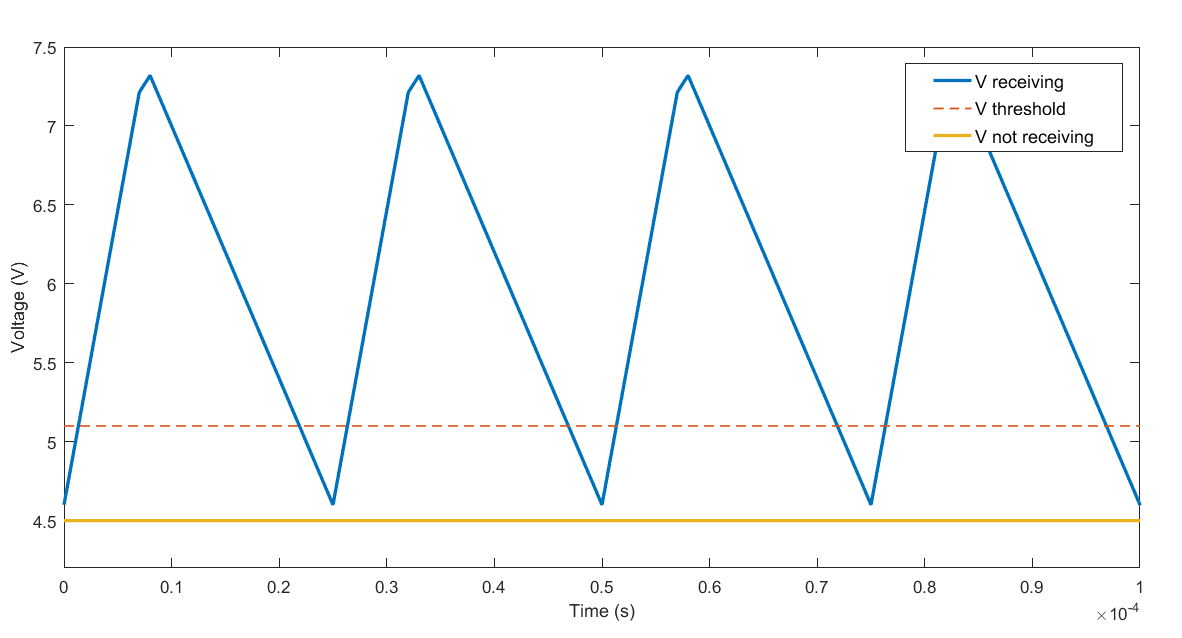
\includegraphics[width=0.9\textwidth]{Figures/waves_peak_detect_test.png}
\caption{Effect of a high peak to peak voltage output of the peak detect circuit}
\label{fig:waves_peak_test}
\end{figure}

When the circuit is receiving we see that the waveform at the output of the peak detection circuit has a higher peak to peak voltage and a lower mean than expected.
Due this high peak to peak voltage the signal at the input of the comparator goes below the threshold voltage each capacitor charge-discharge cycle (see Figure~\ref{fig:waves_peak_test}).
Thus the signal at the output, $US_{detect}$, is constantly switching between the high (not receiving) and low (receiving) state.
This can be solved by making some modification to the component values in the peak detection circuit.
The modifications made to the amplifiers and the peak detection circuit will be discussed in the next section.


\subsection{Modifications}
\label{chap:mod}
As discussed in the previous section the first prototype did not have the desired results. The first operational amplifiers produces a small oscillating signal which is amplified by the second stage op-amp. This oscillating signal could come from the resistor capacitor combination before the first op-amp or by the low bandwidth, gain bandwidth product of the LM741's. The voltage gain falls rapidly with increasing the signal frequency. At 40 kHz the gain of the LM741 is only 25 times. The LM741's are made for sound amplification that has a maximum at 22 kHz The replacement operational amplifier, the LF353 \cite{LF353}, has a higher bandwidth which results in a higher possible voltage gain. With this modification the noise oscillation, as discussed in the previous section, is not noticeable any more. So this modification fixed the low gain and distortion signal for the peak detection circuit.

The problem with the peak detection circuit came from the fact that the capacitor discharges to fast. This is solved to change the discharge resistor to a higher value\footnote{The final values of the resistor is given in the circuit of appendix \ref{Appendixcircuits}.}, this way the capacitor discharges slower and the output signal of the peak detection circuit doesn't fall underneath the $V_{th}$ anymore.


\subsection{Results after modifications}

Figure~\ref{fig:proof_test_1} gives the results for the set-up without obstacles or reflections.
In this case there is a clear difference between the high and low state which can be detected by the micro controller.

\begin{figure}[H]
\centering
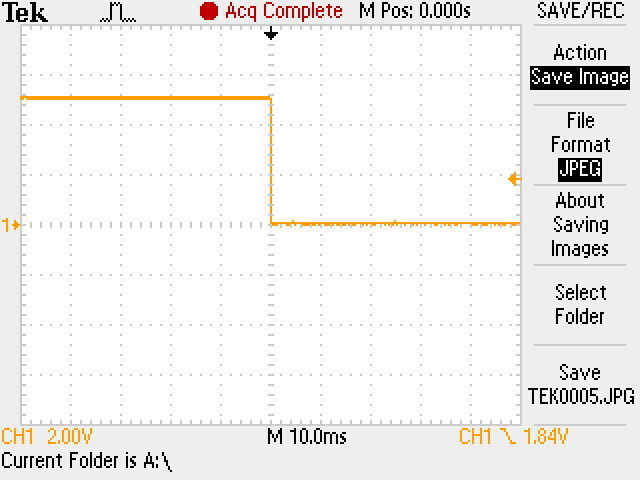
\includegraphics[width=0.6\textwidth]{test_proof_1.JPG}
\caption{Proof of concept test of US detect signal in direct orientation}\label{fig:proof_test_1}
\end{figure}

If the transmitter and receiver are placed in a less favourable set-ups with reflections and obstacles.
The low state of the $US_{detect}$ signal is not always stable. %cancellation
Due to the reflections and obstacles the transducer does not receive the entire pulse, either because parts are blocked or have destructive interferences from the multiple paths caused by the reflections.
This instability might cause measurements to fail or become inaccurate since the micro controller might see the signal as high instead of the low corresponding to receiving.
We estimate the effect of this instability to be negligible since:

\begin{itemize}
\item
Only the first falling edge is important, this is the most direct path the ultrasonic signal travels. The distortions mostly result out of reflections and signal cancellations, but these signals are never the direct path of the signal. This is why these instabilities can be neglected.
\item
Since we want to have an accuracy of 10cm over the distance of 1 meter. We need to poll at a certain frequency. The speed of sound is \SI{343}{\meter}$s^{-1}$, the time it takes for sound to travel 10 cm is 0.29ms. This is why we will use a clock of \SI{40}{\kilo\hertz} for the polling, this frequency does have period of 0.025ms and thus can reach an accuracy of $343 * 0.025 = 8.6 mm$ in ideal conditions.
The received noise is in the order of mili seconds. This means that we might do a miscount due to the noise but the error will be in the order of \SI{25}{\micro\second}.
To miss an entire measurement the noise would have to perfectly align with the counter cycle such that the signal is high every time the counter checks the $US_{detect}$ signal.
We assume the chances for this to happen are low but at this point in time we cannot yet measure the influence of the noise since the communication subsystem and micro controller are not yet integrated.
As soon as we have a working system prototype, with all subsystems integrated, we can test how often a measurement fails due to the noise.
\item
Since the speed of the Zebro is low, \SI{5}{\meter\per\second}, and the frequency of measurements is high a neighbouring Zebro will not have moved out of communication range when one measurement is failed.
It is not necessary to know the accurate location of each neighbour as long as the Zebro know that he is within communication range of others.
\item
The processing method, a particle filter, has capabilities to detect missed measurements and to act accordingly. \cite{processing}
\end{itemize}

\begin{figure}[H]
\centering
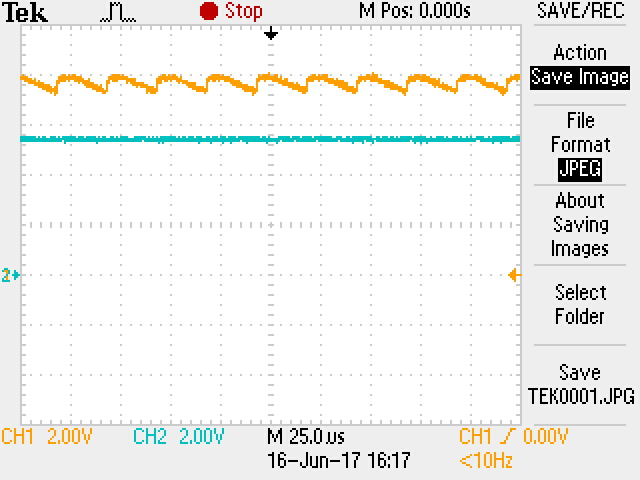
\includegraphics[width=0.6\textwidth]{Vth_Vpeak.JPG}
\caption{Peak detect signal together with the $V_{th}$ of the first comparator when receiving}\label{fig:peakvth}
\end{figure}

The peak detection circuit was also being modified and gives a much better result now. As can be seen in Figure \ref{fig:peakvth}, the peak detect signal (Yellow) stays high when receiving a pulse the capacitor discharges slowly enough to keep the signal above the $V_{th}$ (Blue) of the first comparator. The zero reference is turned 1 division down to get a better plot. So the $V_{th}$ is around 5.2V.

As discussed in section \ref{sec:antenna_proof} the risers of the antenna could give the antenna a blind spot, however with testing we didn't recognise any influence on the transmitter and receiver side due to these risers.

\section{Conclusion}
From the test we have done we can conclude that the transmitter and receiver concept prototypes work after the needed modifications. The task now is to combine the both circuits to a working prototype.
The antenna works properly as well as we can see from the results. With simple test the range of the transmitter and receiver can reach easily 5 meters.
The only remark that can be made is that the both comparators don't have hysteresis implemented yet. This is done because the $V_{th}$ of the first comparator is close to the voltage of the not receiving signal. This results in the situation that the hysteresis region becomes small. This is why in this stage of the project is chosen to leave the hysteresis in the comparators away.
